\chapter{Infinity and missing values}
\thispagestyle{fancy}
\label{ch:infinity-etc}



Since a computer is a discrete and finite machine, certain operations are undefined:
\begin{action}
Type 
\prompt{10/0}
\end{action}
The result of this operation is {\tt Inf}\index{Inf@\texttt{Inf}}. {\tt Inf} is the arithmetic representation for positive infinity ({\tt -Inf} for negative infinity). Infinity results from operations like division by zero and overflow (calculations that lead to results too large to represent as conventional floating-point values).
\begin{action}
Type 
\prompt{0.0/0.0}
\end{action}
The result of this (illegal) operation is {\tt NaN}\index{NaN@\texttt{NaN}}: Not-a-Number. A {\tt NaN} result is obtained because of mathematically undefined operations. Undefined operations that produce {\tt NaN}: 
\begin{enumerate}
\item any arithmetic operation on an array containing {\tt NaN}
\item division, such as {\tt 0/0} and {\tt Inf/Inf}
\end{enumerate}
Often {\tt NaN}s occur in imported data.
\begin{action}
Type
\prompt{A = [1,2,3;4,NaN,6;7,8,9]}
\end{action}
\begin{action}
Try to calculate the mean and standard deviation of {\tt A}.
\end{action}
Because arithmetic operations on {\tt Inf} or {\tt NaN} produce {\tt Inf} or {\tt NaN}, it is necessary to remove or replace these values in arrays before further calculations.
\begin{action}
Type
\prompt{B = [123,Inf,43.2,18,28,NaN,pi,exp(1),-Inf,4]}\index{pi@\texttt{pi}}
\end{action}
\begin{action}
Type
\prompt{Bnan = isnan(B)}\index{isnan@\texttt{isnan}}
and
\prompt{Binf = isinf(B)}\index{isinf@\texttt{isinf}}
and interpret the results. Take a look at the data classes of the variables listed in the workspace.
\end{action}
\begin{action}
Use {\tt isnan}, {\tt isinf} and {\tt find} in combination with logical and relational operators to create an array {\tt BFinite} that contains only those values of {\tt B} that are not {\tt NaN} or {\tt Inf}. Use only one command line. The result {\tt BFinite} should be an 1x7 array.
\end{action}

\project{Aluminum toxicity}
\label{pr:aluminum-toxicity}
Often, the data you import or create during programming contain errors. Values such as {\tt NaN}, {\tt -Inf}, and {\tt Inf} can occur in a data set as a result of measurement errors or illegal mathematical operations. Because statistical operations are impossible on these values, it is sometimes necessary to remove them from your data before further calculation.

Aluminum (Al) is a common element found in sandy soils. At pHs up to about 4.5, Al$^{3+}$ is the most common form of Al. At higher pHs, the Al can form complexes and become immobile in the soil environment. The `free' Al$^{3+}$-ion is mobile and can be transported easily with the soil water. This way plants can take up Aluminum, which is an important nutrient. However, high Al$^{3+}$ concentrations can become toxic to plants, inhibiting growth or even causing death. Evaluating concentrations of Al$^{3+}$ is important in determining the toxicity hazards in ecosystems. In the Dutch dunes, many experiments have taken place that monitor Al$^{3+}$ concentrations in the soil water. We have obtained the data of one of these experiments, which we will use for the following exercises.

\begin{action}
Set your work directory to `\textbackslash{}ch10\_inf\_nan\textbackslash{}proj05\_al\_tox' and start a new script called `\starred{name}\_al\_tox' (in which \starred{name} is your last name). Let the script load and visualize the data from the file `al\_conc.txt'. This file contains data on daily concentration of Al$^{3+}$ in soil water for a period of 365 days. Call the new variable {\tt AlConc} using:
{\tt AlConc=load(\squote{al\_conc.txt})}
\end{action}
As you can see, the data contains outliers (extreme values due to measuring errors or extreme conditions), {\tt NaN}s and zero values where measurement errors have occurred.

To get a more accurate picture of the trend of the Al$^{3+}$ concentration over time, the data must be filtered. In this project, you will:
\begin{enumerate} 
\item replace {\tt NaN}s and zero values with the mean of surrounding values;
\item calculate the moving average\index{moving average} (MA) of the Al$^{3+}$ concentration over time.
\end{enumerate}
The MA is calculated as the mean of the value itself and a predetermined number of neighboring elements to the left and right of this value. For instance, the 3-term MA at time step 24 is calculated based on the mean of the values of time step 23, 24, and 25. The data is thus smoothed, making it easier to spot trends in the data. For this project, we will calculate the 9-term MA for the {\tt AlConc} array. At the end, the original data, the data without outliers and the smoothed data are all displayed.

Create a flow diagram of how you think you can tackle the problem. If you are confident that you can solve the problem, feel free to use your flow diagram and ignore the steps explained below (You can always come back here for a step by step approach if your plan didn't work out). 
\begin{action}
First, alter your script so that the {\tt AlConc} data is visualized in the first subplot of a figure with three subplots beneath each other.
\end{action}
\begin{action}
Create two logical arrays: the first which is true at the locations where the concentration is zero, the second is true where there are {\tt NaN}s. Assign your variables sensible names.
\end{action}
\begin{action}
Combine these two arrays with a logical expression and then use the {\tt find} function to identify the indices of the locations that need to be interpolated.
\end{action}

Instead of replacing these zeros and NaNs with a predetermined value, we have to calculate the mean of the 2 cells surrounding the corrupt value. Because this has to be done for multiple elements, the use of a loop is required.

Write the loop that calculates the new value for all elements of an array {\tt AlConcFilled} that you must create. The easiest way to do so is in these steps:
\begin{enumerate}
\item Copy the contents of {\tt AlConc} to your new variable {\tt AlConcFilled}.
\item Create the statement that calculates the new value to replace the {\tt 0} or {\tt NaN} at a given index, based on the two neighboring cells. 
\item Make the statement more generic by expressing the previous step in terms of a variable rather than numbers.
\item Use a {\tt for}-loop to iterate over the indexes that need to be changed.
\end{enumerate}
If you like, you can also avoid a {\tt for}-loop altogether and perform your calculations using a vectorized way of programming (see page~\pageref{ind:vectorization}).
\begin{action}
Is this method valid for any distribution of zeros and {\tt NaN}s within an array? Why or why not? If you think not, give an example where the method would not be able to calculate a valid mean value to replace a zero or {\tt NaN}.
\end{action}
\begin{action}
Can you think of a way to solve the shortcoming? Describe the principle in words or in command lines.
\end{action}
For calculating the moving average, we can use a similar method as for the filling process we used to make {\tt AlConcFilled}. The 9-term MA is calculated based on the 4 array elements to the left, 4 array elements to the right, as well as the middle element. For the next exercise, you need to copy and paste the loop you used to calculate {\tt AlConcFilled}, and adapt it to calculate a new array {\tt AlConcMA9}, which contains the 9-term moving average of Aluminum concentrations.
\begin{action}
For {\tt AlConcFilled}, we iterated over the holes in the data, but for {\tt AlConcMA9}, this works differently. Adapt the {\tt rowvector} bit (see page~\pageref{ind:rowvector}).
\end{action}
\begin{action}
Inside the loop, adapt your command to calculate the average of the 4 array elements to the left, 4 array elements to the right, and the middle element.
\end{action}
\begin{action}
Display the final {\tt AlConcMA9} in subplot 3 in the figure. Add a title and label the axes.
\end{action}
\begin{action}
Does {\tt AlConcMA9} structurally over- or underestimate the Al$^{3+}$ concentration? How did you check this?
\end{action}
\begin{action} 
The threshold between toxic and non-toxic Al$^{3+}$ concentrations is 70~$\mu{}$mol/L. If the {\tt AlConcMA9} data is used, will this underestimate or overestimate the period in a year in which toxic Al$^{3+}$ levels are reached?
\end{action}
\noindent So, even though the MA offers more insight in the trend in a certain data series, it can underestimate hazards because extreme values are filtered.
\begin{action}
Alter the program in such a way, that the number of terms for calculation of the MA can be set dynamically. The program user has to be able to change the calculation to a 5, 11, or 15-term MA by changing one value in the initialization part of your program (see page~\pageref{ind:initialization-part}).
\end{action}
\begin{action}
In addition to the MA line in subplot 3, use magenta dots to visualize the data from {\tt AlConcFilled}. Refer to Project ``Columbia river'' on page~\pageref{pr:columbia} if you forgot how to visualize multiple data sets in one figure.
\end{action}
If your script works correctly, it should yield a picture like that of Figure~\ref{fig:aluminum-concentration}.
\begin{figure}[!htb]
  \centering
    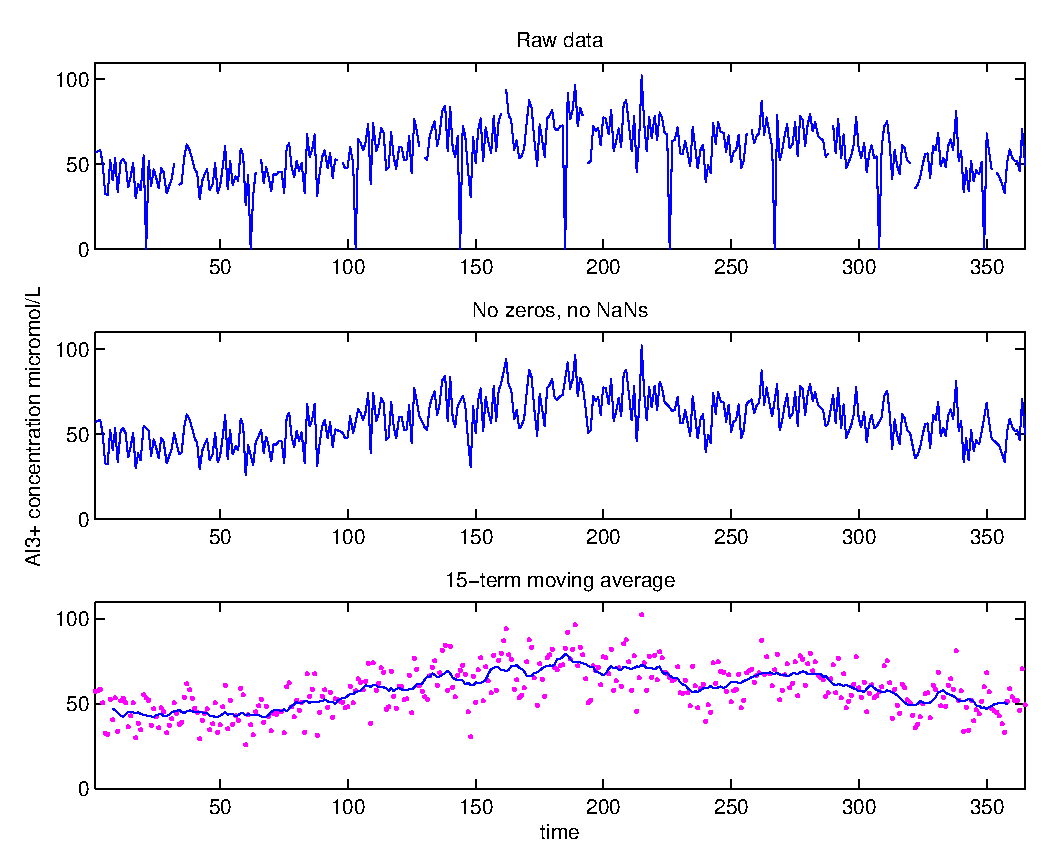
\includegraphics[width=1.0\textwidth]{./../eps/aluminum-concentration.eps}
  \caption{End result of Project \ref{pr:aluminum-toxicity}.}\label{fig:aluminum-concentration}
\end{figure}

